% Options for packages loaded elsewhere
\PassOptionsToPackage{unicode}{hyperref}
\PassOptionsToPackage{hyphens}{url}
%
\documentclass[
]{article}
\usepackage{amsmath,amssymb}
\usepackage{iftex}
\ifPDFTeX
  \usepackage[T1]{fontenc}
  \usepackage[utf8]{inputenc}
  \usepackage{textcomp} % provide euro and other symbols
\else % if luatex or xetex
  \usepackage{unicode-math} % this also loads fontspec
  \defaultfontfeatures{Scale=MatchLowercase}
  \defaultfontfeatures[\rmfamily]{Ligatures=TeX,Scale=1}
\fi
\usepackage{lmodern}
\ifPDFTeX\else
  % xetex/luatex font selection
\fi
% Use upquote if available, for straight quotes in verbatim environments
\IfFileExists{upquote.sty}{\usepackage{upquote}}{}
\IfFileExists{microtype.sty}{% use microtype if available
  \usepackage[]{microtype}
  \UseMicrotypeSet[protrusion]{basicmath} % disable protrusion for tt fonts
}{}
\makeatletter
\@ifundefined{KOMAClassName}{% if non-KOMA class
  \IfFileExists{parskip.sty}{%
    \usepackage{parskip}
  }{% else
    \setlength{\parindent}{0pt}
    \setlength{\parskip}{6pt plus 2pt minus 1pt}}
}{% if KOMA class
  \KOMAoptions{parskip=half}}
\makeatother
\usepackage{xcolor}
\usepackage[margin=1in]{geometry}
\usepackage{graphicx}
\makeatletter
\def\maxwidth{\ifdim\Gin@nat@width>\linewidth\linewidth\else\Gin@nat@width\fi}
\def\maxheight{\ifdim\Gin@nat@height>\textheight\textheight\else\Gin@nat@height\fi}
\makeatother
% Scale images if necessary, so that they will not overflow the page
% margins by default, and it is still possible to overwrite the defaults
% using explicit options in \includegraphics[width, height, ...]{}
\setkeys{Gin}{width=\maxwidth,height=\maxheight,keepaspectratio}
% Set default figure placement to htbp
\makeatletter
\def\fps@figure{htbp}
\makeatother
\setlength{\emergencystretch}{3em} % prevent overfull lines
\providecommand{\tightlist}{%
  \setlength{\itemsep}{0pt}\setlength{\parskip}{0pt}}
\setcounter{secnumdepth}{-\maxdimen} % remove section numbering

%\newcommand{\beginsupplement}{%
%        \setcounter{table}{0}
%        \renewcommand{\thetable}{\arabic{table}}%
%        \setcounter{figure}{0}
%        \renewcommand{\thefigure}{\arabic{figure}}%
%     }

\newcommand{\beginsupplement}{
	\renewcommand{\figurename}{Supplementary Figure}
	\setcounter{figure}{0}
}

%\usepackage{xr}
%\externaldocument{Supplementary_File1}

\usepackage{lineno}
\linenumbers

\usepackage[compress, super]{natbib}

\usepackage{setspace} \doublespacing

\usepackage{siunitx}

\usepackage[utf8]{inputenc}
\usepackage{amsmath}
\usepackage{algorithm}
\usepackage{algpseudocode}

\algrenewcommand\algorithmicrequire{\textbf{Input:}}
\algrenewcommand\algorithmicensure{\textbf{Output:}}
\ifLuaTeX
  \usepackage{selnolig}  % disable illegal ligatures
\fi
\IfFileExists{bookmark.sty}{\usepackage{bookmark}}{\usepackage{hyperref}}
\IfFileExists{xurl.sty}{\usepackage{xurl}}{} % add URL line breaks if available
\urlstyle{same}
\hypersetup{
  pdftitle={Figure Testing for: Transcripts with high distal heritability mediate genetic effects on complex metabolic traits},
  hidelinks,
  pdfcreator={LaTeX via pandoc}}

\title{Figure Testing for: Transcripts with high distal heritability
mediate genetic effects on complex metabolic traits}
\author{}
\date{\vspace{-2.5em}}

\begin{document}
\maketitle

\begin{figure}[ht!]
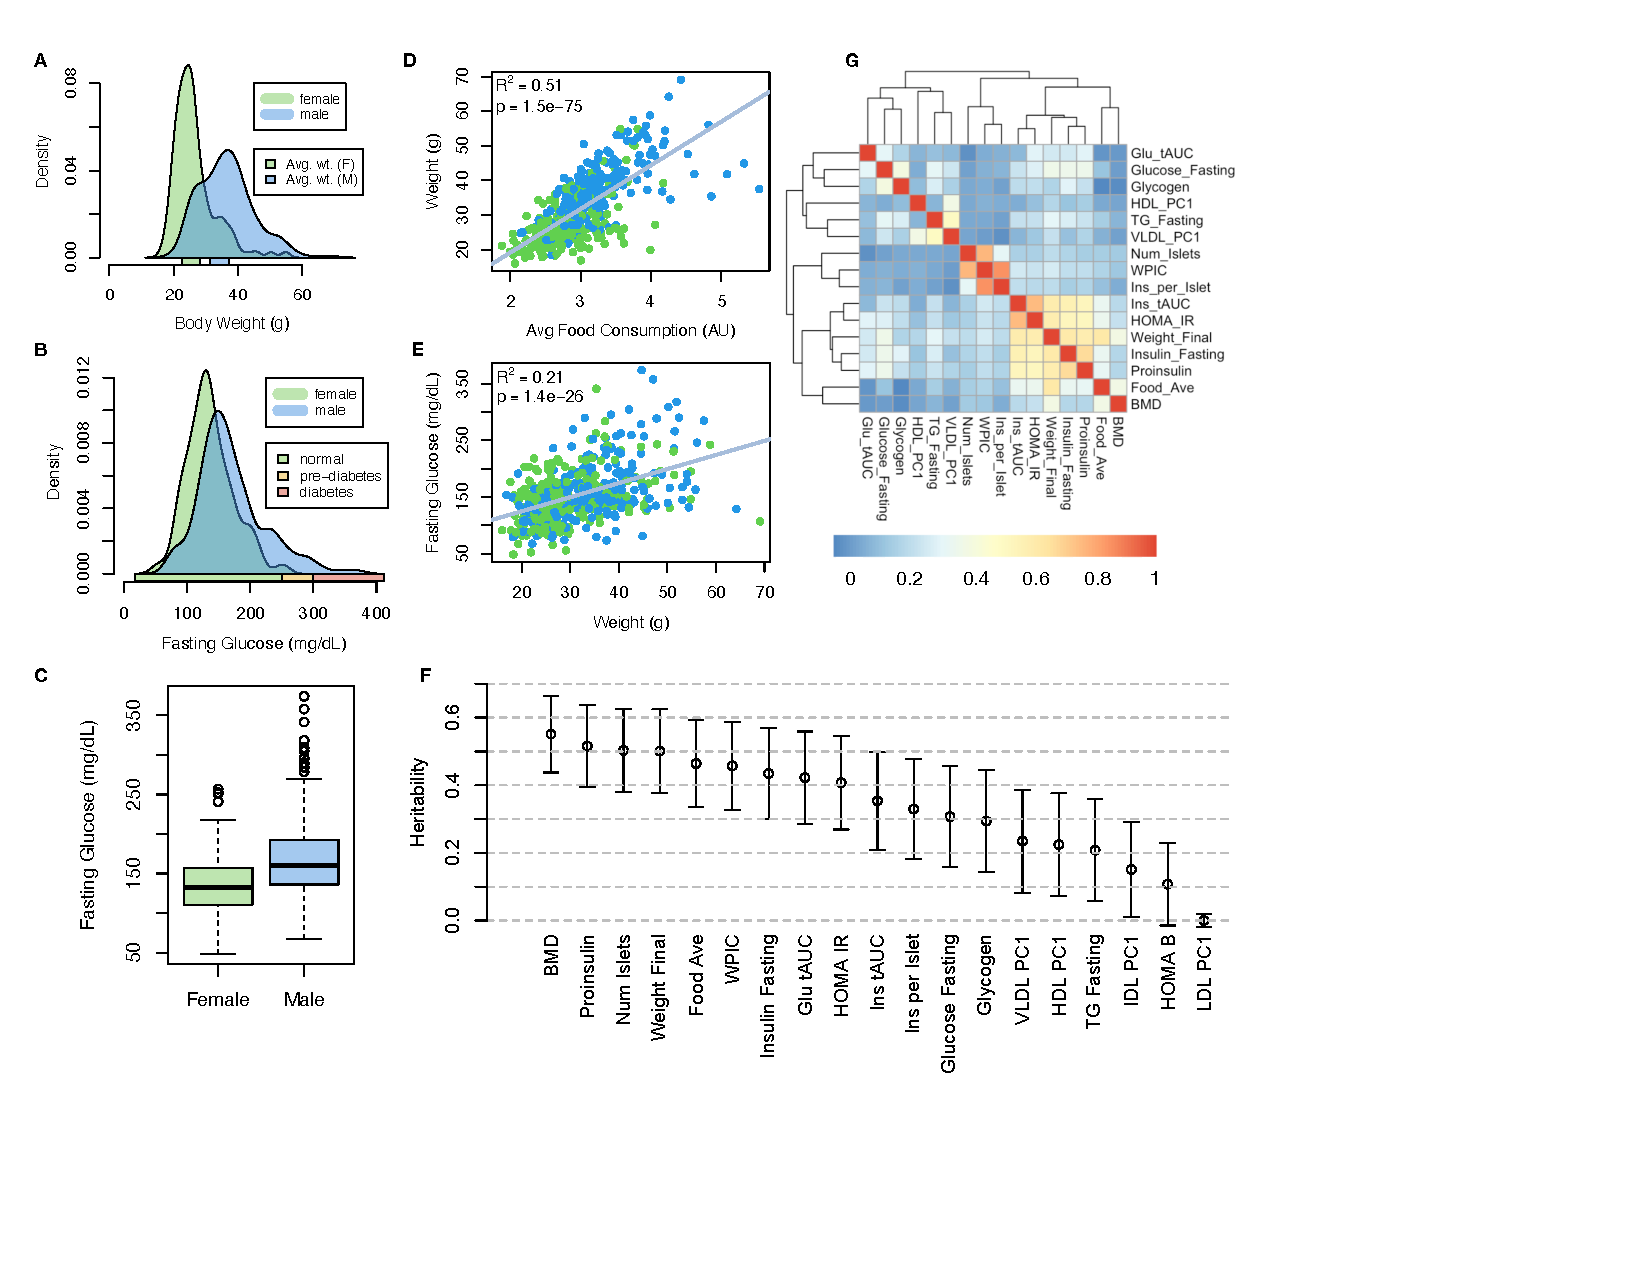
\includegraphics[width=\textwidth]{Figures/Fig1_trait_overview.pdf} 
\caption{ Clinical overview. \textbf{A.} Distributions of final body 
weight in the diversity outbred mice. Sex is indicated by color. 
The average B6 male and female adult weights at 24 weeks of 
age are indicated by blue and green bars on the x-axis. \textbf{B.} 
The distribution of final fasting glucose across the population split 
by sex. Normal, pre-diabetic, and diabetic fasting glucose levels for 
mice are shown by colored bars along the x-axis. \textbf{C.} Males 
had higher fasting blood glucose on average than females 
($p = 9.1\times10^{-15}$). \textbf{D.} The relationship between 
food consumption and body weight for both sexes. \textbf{E.} 
Relationship between body weight and fasting glucose for both 
sexes. \textbf{F.} Heritability estimates for each physiological trait. 
Bars show standard error of the estimate. \textbf{G.} Correlation 
structure between pairs of physiological traits. The lower triangle 
shows Pearson correlation coefficients between pairs of traits (r). 
The upper triangle shows the Pearson correlation coefficient (r) 
between LOD traces of pairs of traits, and diagonal shows the 
estimated heritability of each trait. BMD - bone mineral density,
WPIC - whole pancreas insulin content, Glu tAUC - glucose total area under 
the curve, HOMA IR - homeostatic measurement of insulin resistance, HOMA B - 
homeostatic measure of beta cell health, VLDL - very low-density lipoprotein,
LDL - low-density lipoprotein, IDL - intermediate density lipoprotein, 
HDL - high-density lipoprotein, TG - triglyceride.
}
\label{fig:trait_overview}
\end{figure}

\begin{figure}[ht!]
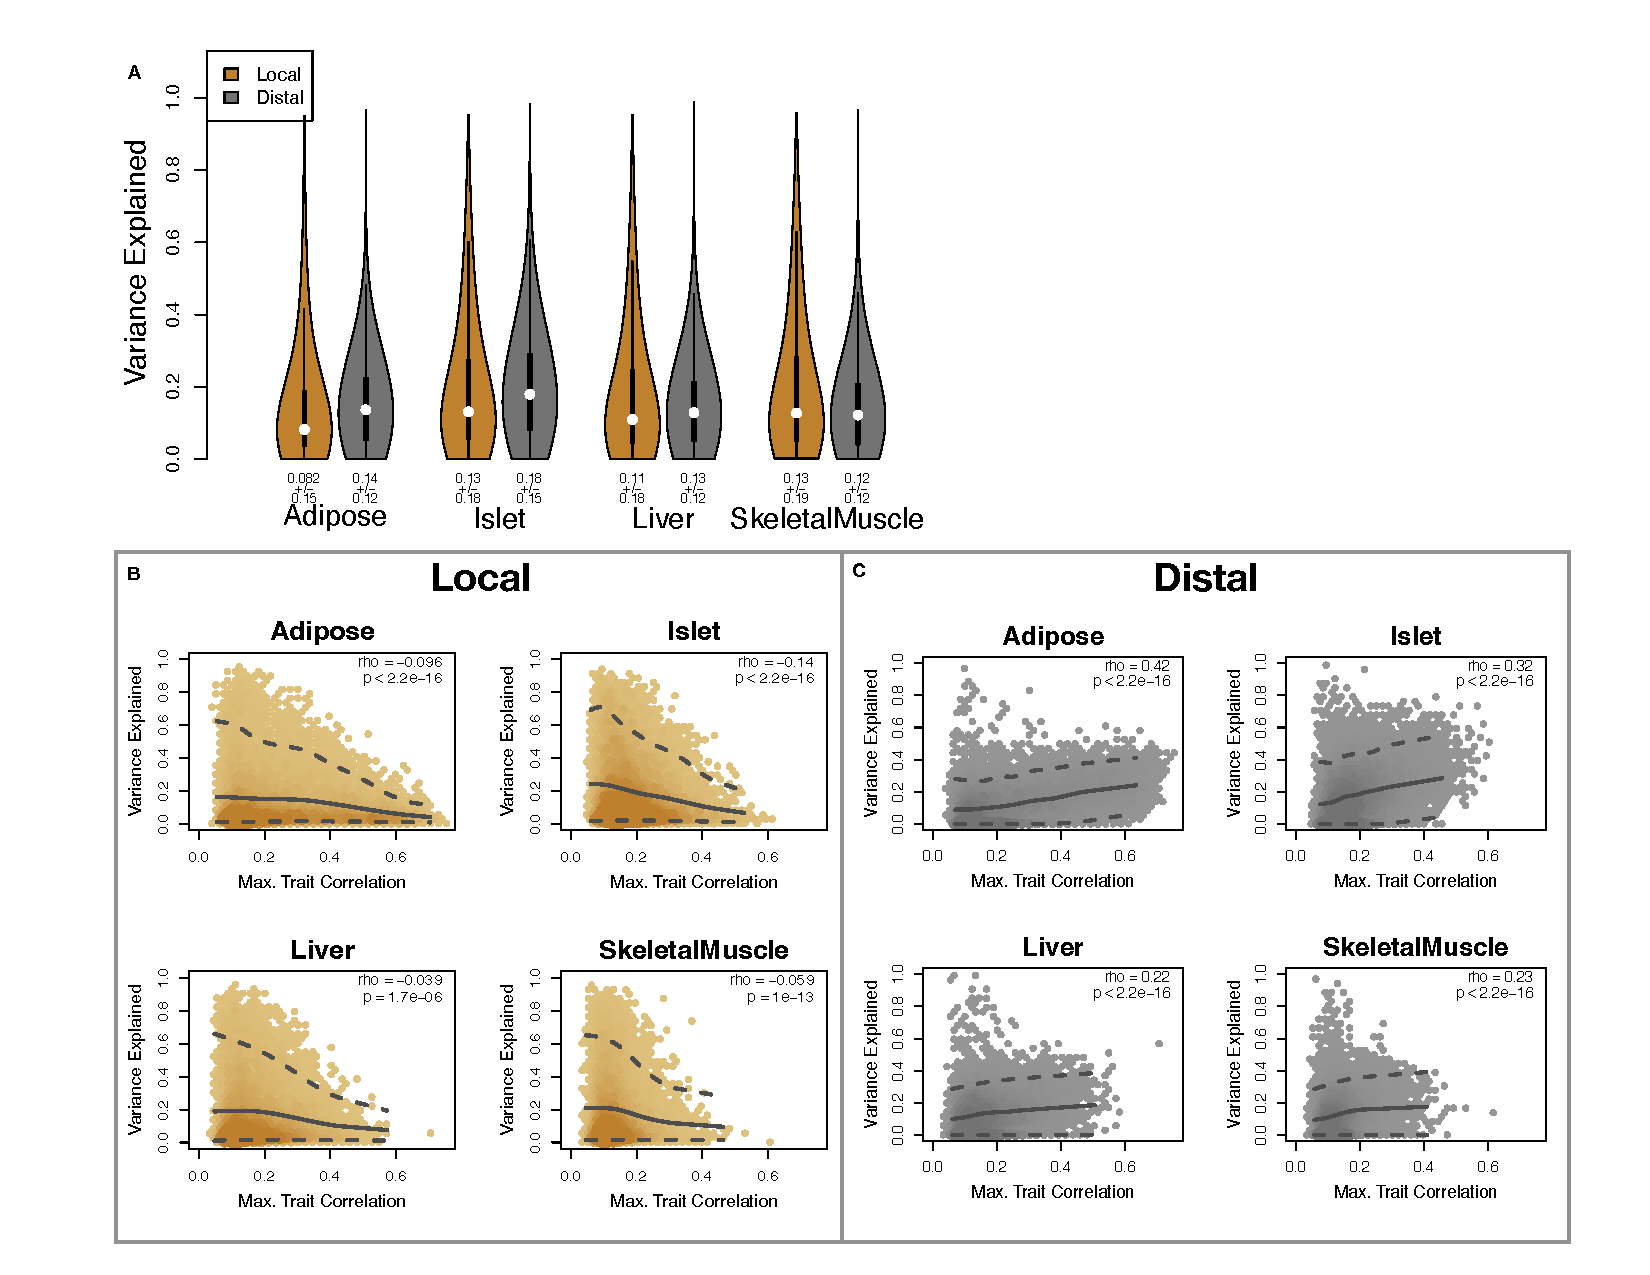
\includegraphics[width=\textwidth]{Figures/Fig2_motivation.pdf} 
\caption{Transcript heritability and trait relevance. 
\textbf{A.} Distributions of local and distal heritability 
of transcripts across the four tissues. Overall local and 
distal factors contributed equally to transcript heritability. 
The relationship between (\textbf{B.}) local and (\textbf{C.}) 
distal heritability and trait relevance across all four 
tissues. Here trait relevance is defined as the maximum 
correlation between the transcript and all traits. The upper 
and lower dashed line in each panel show the 95th and 5th 
percentile correlation. The solid line shows the mean trait 
correlation in transcripts with increasing variance explained 
either locally (B) or distally (C). Transcripts that are highly 
correlated with traits tended to have low local heritability and 
high distal heritability.}
\label{fig:motivation}
\end{figure}

\begin{figure}[ht!]
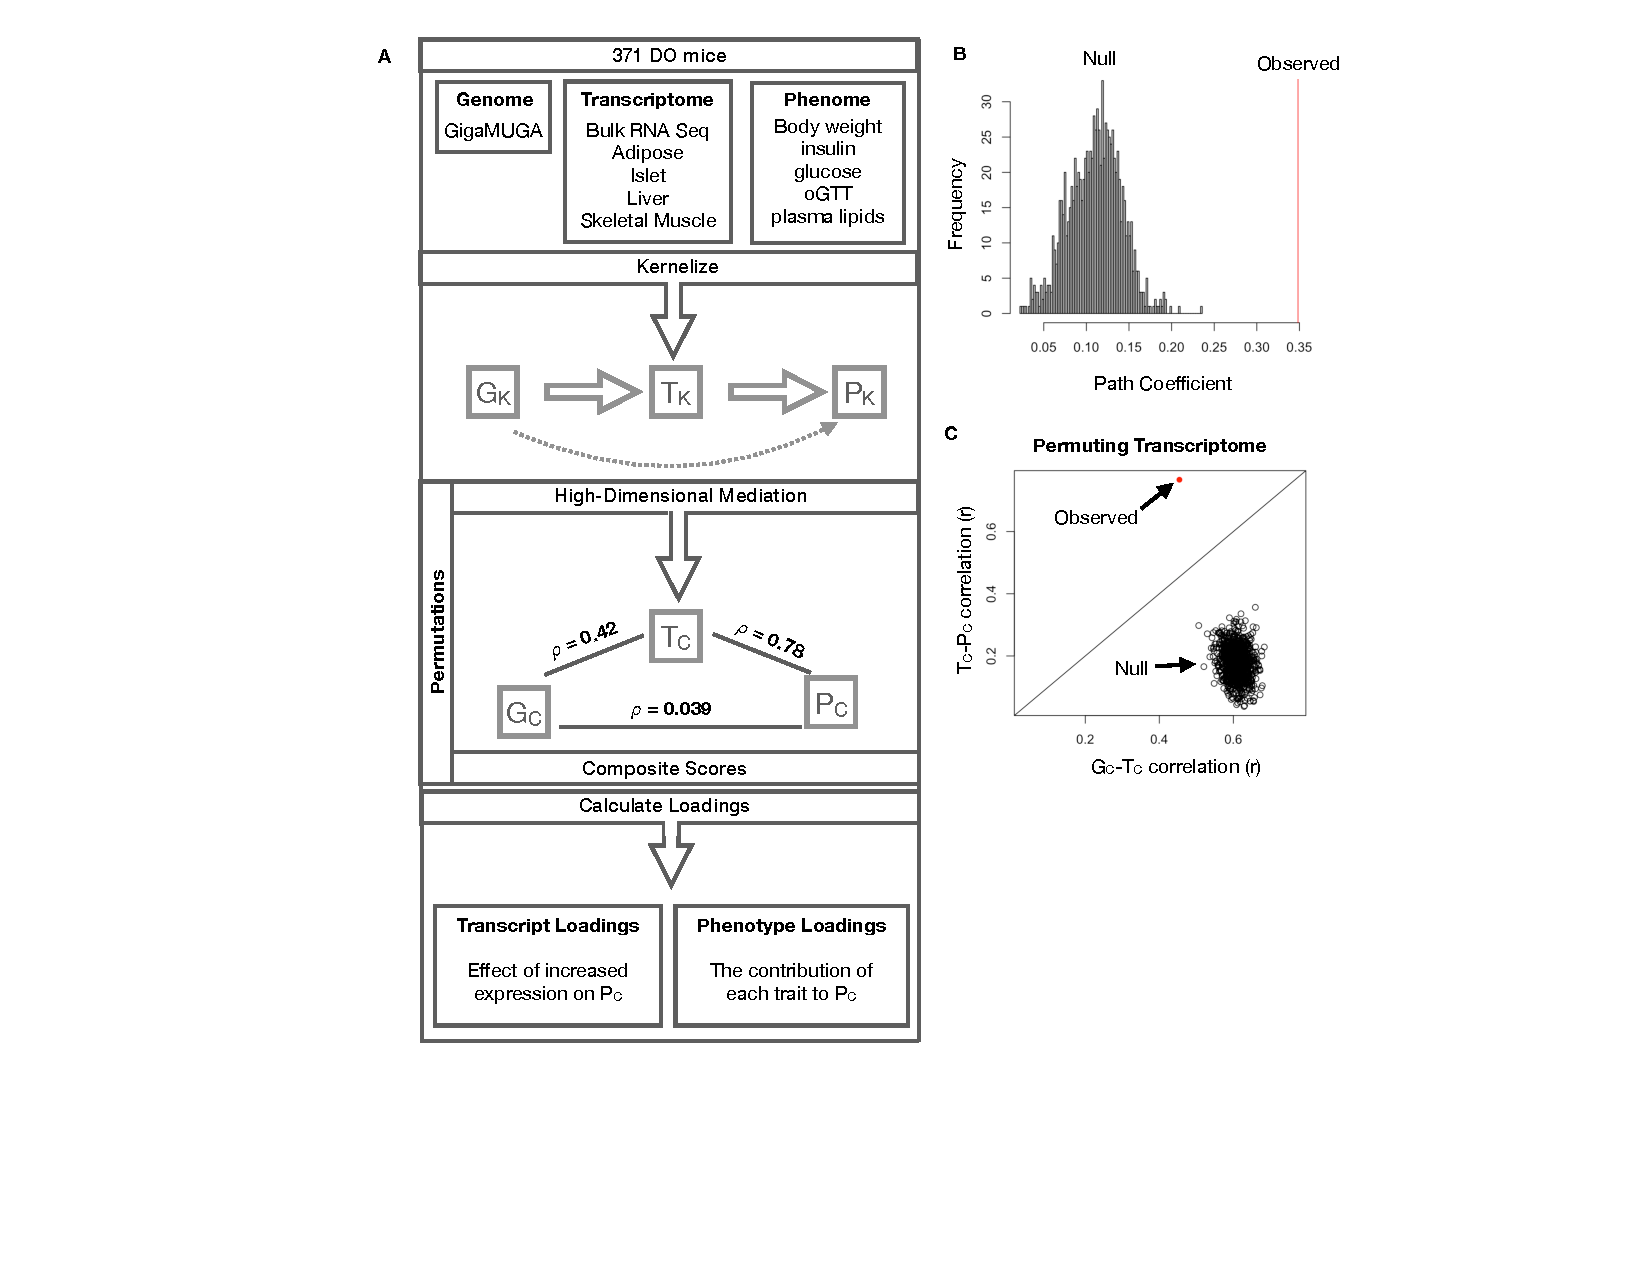
\includegraphics[width=5in]{Figures/Fig3_workflow.pdf} 
\caption{High-dimensional mediation. \textbf{A.} Workflow 
indicating major steps of high-dimensional mediation. The 
genotype, transcriptome, and phenotype matrices were 
kernelized to yield single matrices representing the 
relationships between all individuals for each data modality 
($G_K$ = genome kernel, $T_K$ = transcriptome kernel; 
$P_K$ = phenome kernel). High-dimensional mediation 
was applied to these matrices to maximize the direct path 
$G \rightarrow T \rightarrow P$, the mediating pathway 
(arrows), while simultaneously minimizing the direct $G 
\rightarrow P$ pathway (dotted line). The composite 
vectors that resulted from high-dimensional mediation 
were $G_c$, $T_C$, and $P_C$. The partial correlations 
$\rho$ between these vectors indicated perfect mediation. 
Transcript and trait loadings were calculated as described 
in the methods. \textbf{B.} The null distribution of the path 
coefficient derived from 10,000 permutations. The observed model
(red) is compared to models derived from exclusively distal 
(gray) or local genetic effects (brown). The similarity of 
the observed and distal models indicates the full model is 
dominated by distal genetic effects. \textbf{C.} 
The null distribution of the $G_C$-$T_C$ correlation vs. 
the $T_C$-$P_C$ correlation. Comparisons are shown 
to the observed values (red), and those derived from the 
distal-only model (gray) and the local-only model (brown).
}
\label{fig:workflow}
\end{figure}

\begin{figure}[ht!]
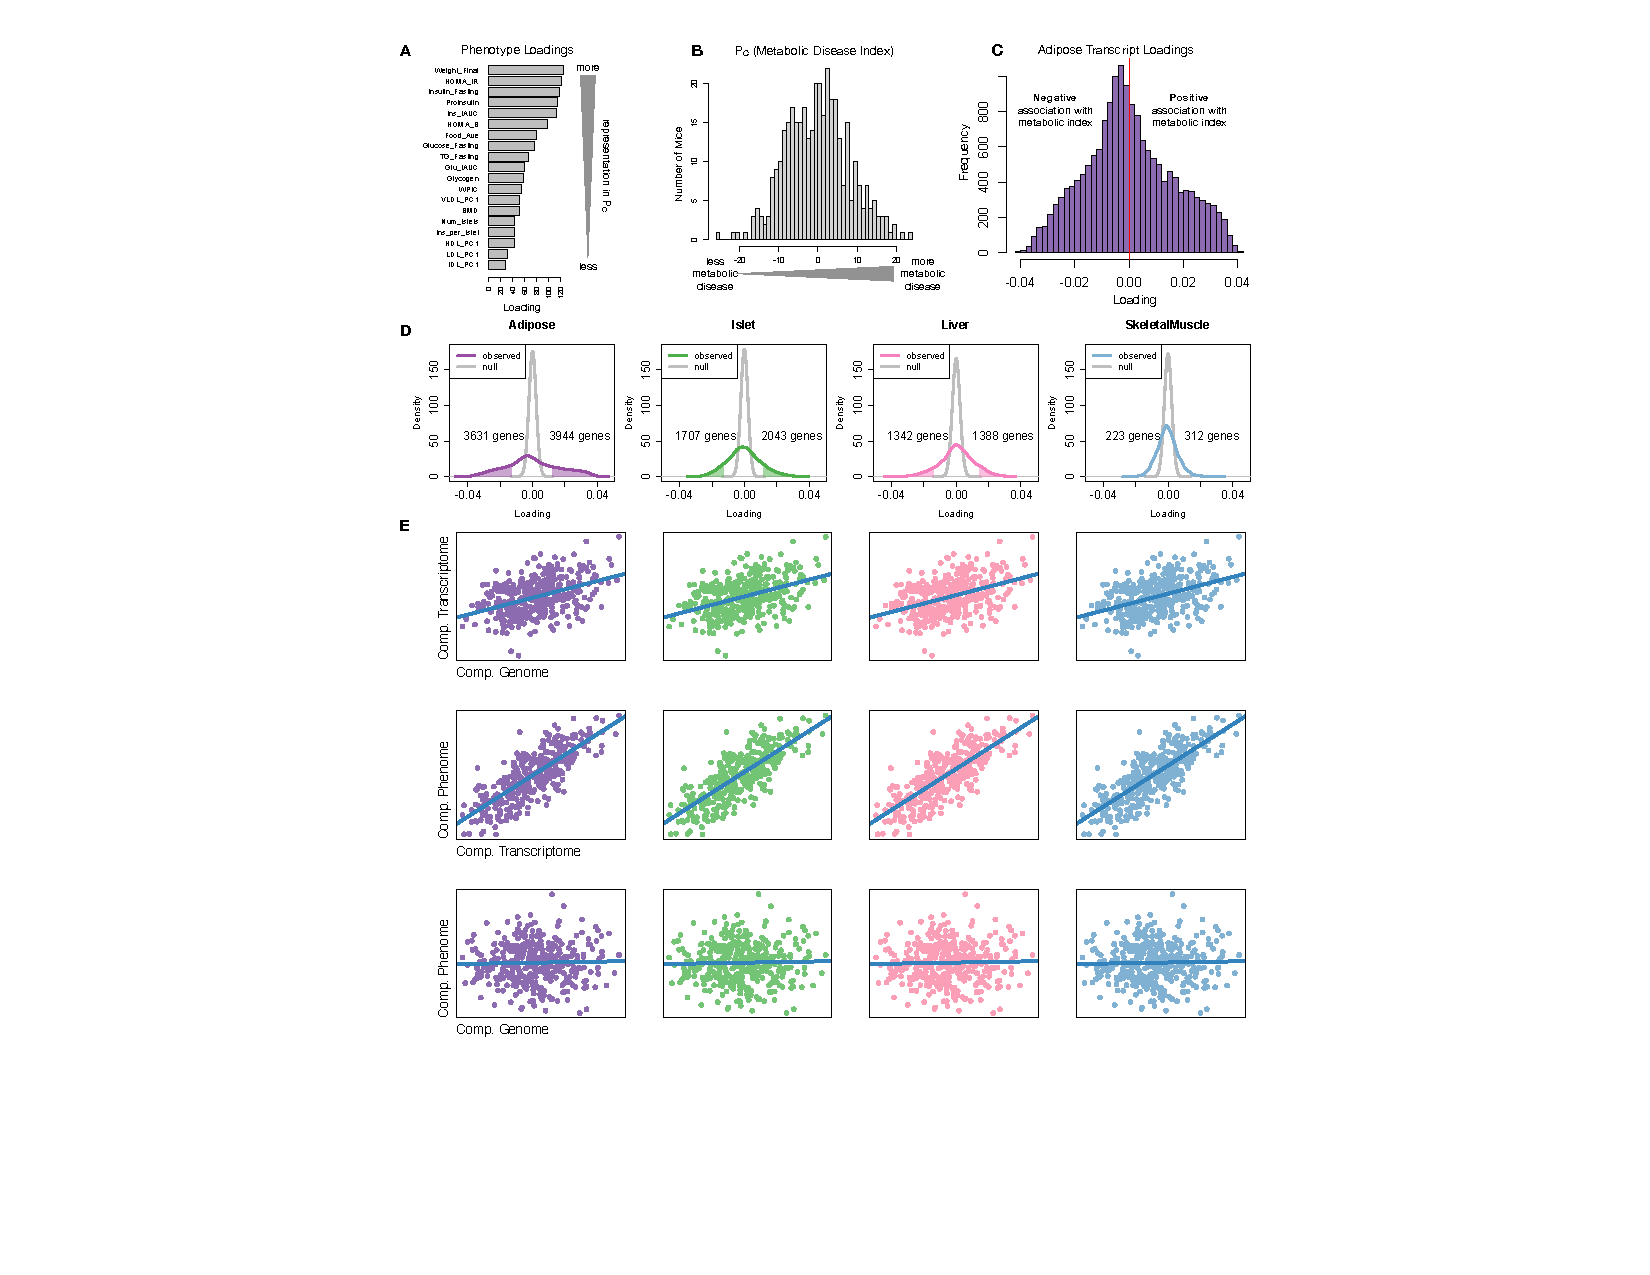
\includegraphics[width=\textwidth]{Figures/Fig4_interpretation.pdf} 
\caption{Interpretation of loadings. \textbf{A.} Loadings across traits. 
Body weight and insulin resistance contributed the most to the composite 
trait. \textbf{B.} Phenotype scores across individuals. Individuals with large 
positive phenotype scores had higher body weight and insulin resistance 
than average. Individuals with large negative phenotype scores had lower 
body weight and insulin resistance than average. \textbf{C.} Distribution of 
transcript loadings in adipose tissue. For transcripts with large positive 
loadings, higher expression was associated with higher phenotype scores. 
For transcripts with large negative loadings, higher expression was associated 
with lower phenotype scores. \textbf{D.} Distributions of loadings across 
tissues compared to null distributions. Shaded areas represent loadings that 
were more extreme than the null distribution. Numbers indicate how many 
transcripts had loadings above and below the extremes of the null. Transcripts 
in adipose tissue had the most extreme loadings indicating that transcripts in 
adipose tissue were the best mediators of the genetic effects on body weight 
and insulin resistance. \textbf{E.} Scatter plots showing correlations between 
composite vectors for the genome ($G_C$), the transcriptome ($T_C$), and the 
phenome ($P_C$). The $G_C$ - $T_C$ correlation is high, the $T_C$ - $P_C$ 
correlation is high, and there is no significant correlation between $G_C$ 
and $P_C$. This correlation structure is consistent with perfect mediation.
}
\label{fig:interpretation}
\end{figure}

\begin{figure}[ht!]
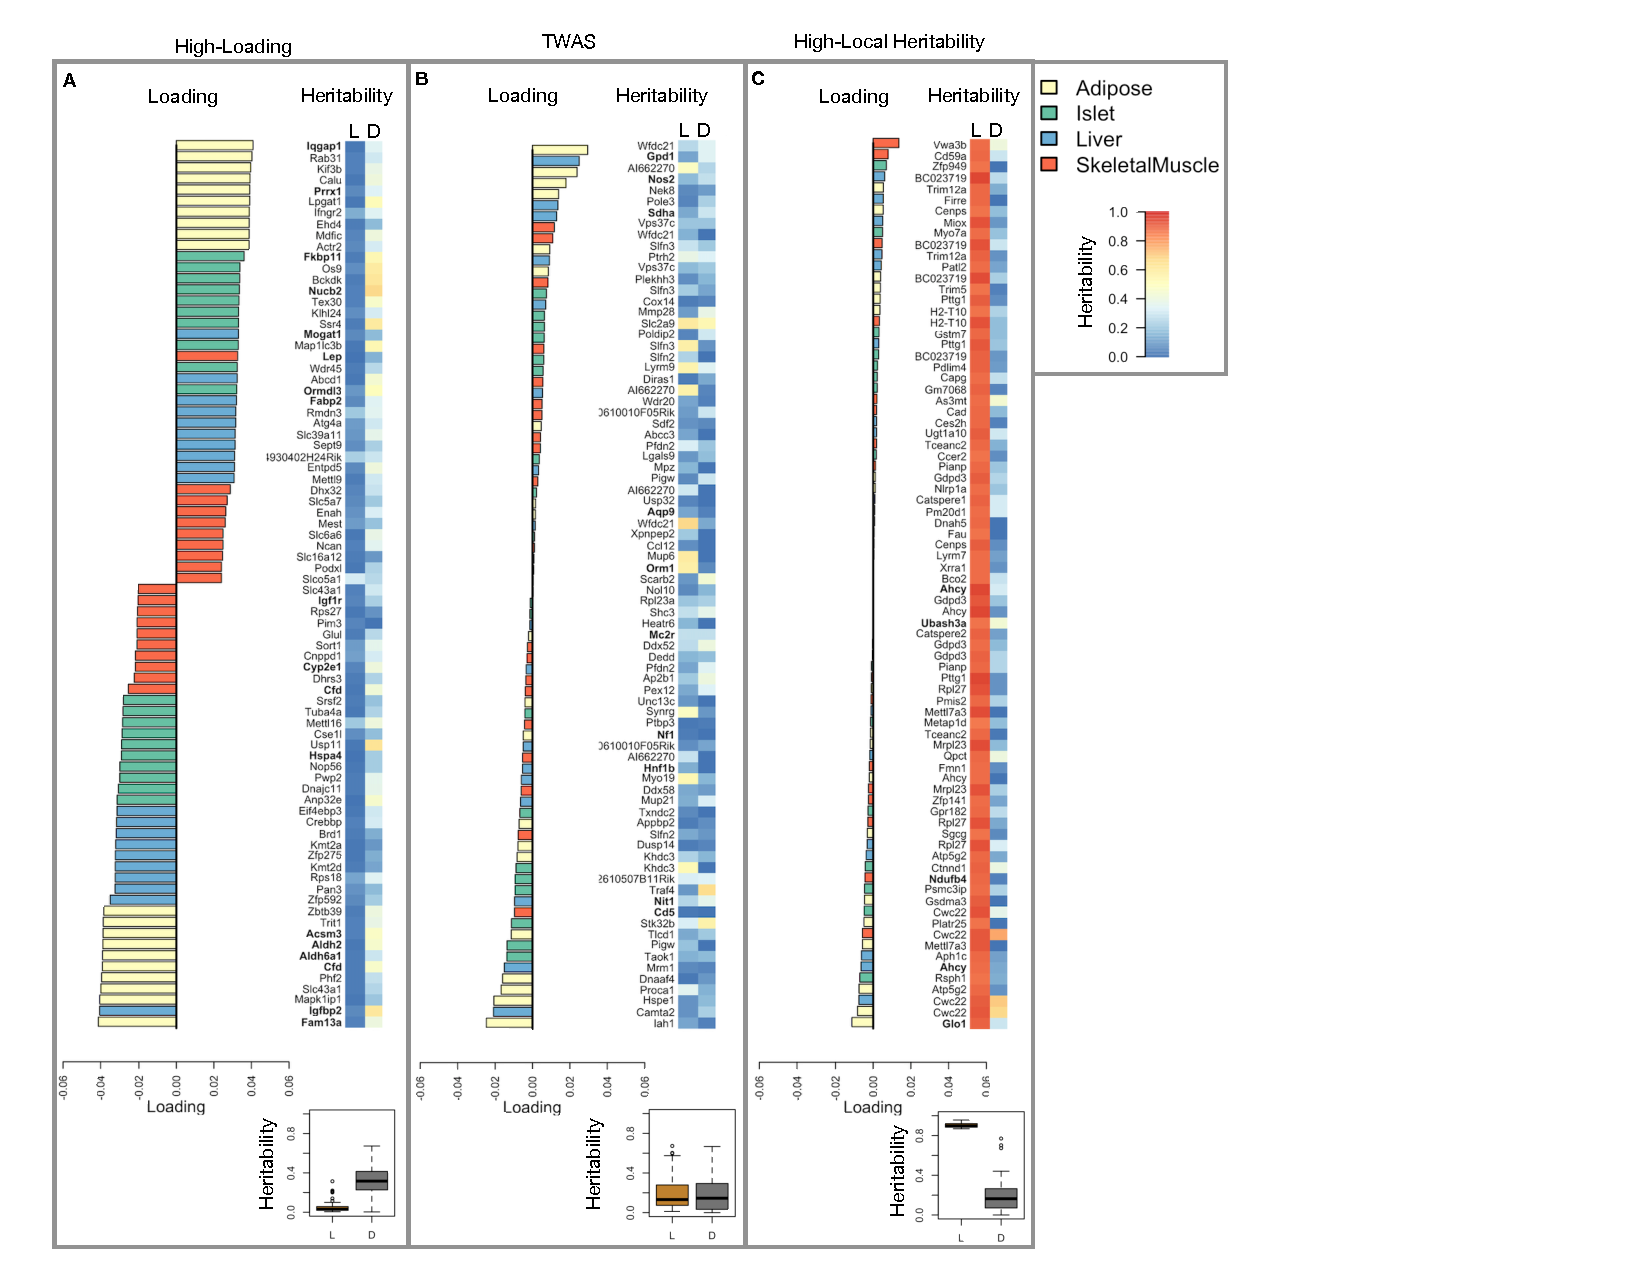
\includegraphics[width=\textwidth]{Figures/Fig5_loading_heritability.pdf} 
\caption{Transcripts with high loadings have high distal heritability 
and literature support (bolded gene names). Each panel has a bar plot 
showing the loadings of transcripts selected by different criteria. Bar color indicates the 
tissue of origin. The heat map shows the local (L - left) and distal 
(D - right) heritability of each transcript. \textbf{A.} Loadings for 
the 10 transcripts with the largest positive loadings and the 10 
transcripts with the largest negative loadings for each tissue. 
Distal heritability was significantly higher than local heritability 
(t-test $p < 2.2^{-16}$). \textbf{B.} Loadings of TWAS candidates 
with the 10 largest positive correlations with traits and the largest 
negative correlations with traits across all four tissues. Local and 
distal heritability were not significantly different for this group 
(t-test $p = 0.77$). \textbf{C.} The transcripts with the largest 
local heritability (top 20) across all four tissues. Local heritability 
was significantly higher than distal heritability of these genes (t-test 
$p < 2.2^{-16}$)
}
\label{fig:loading_heritability}
\end{figure}

\begin{figure}[ht!]
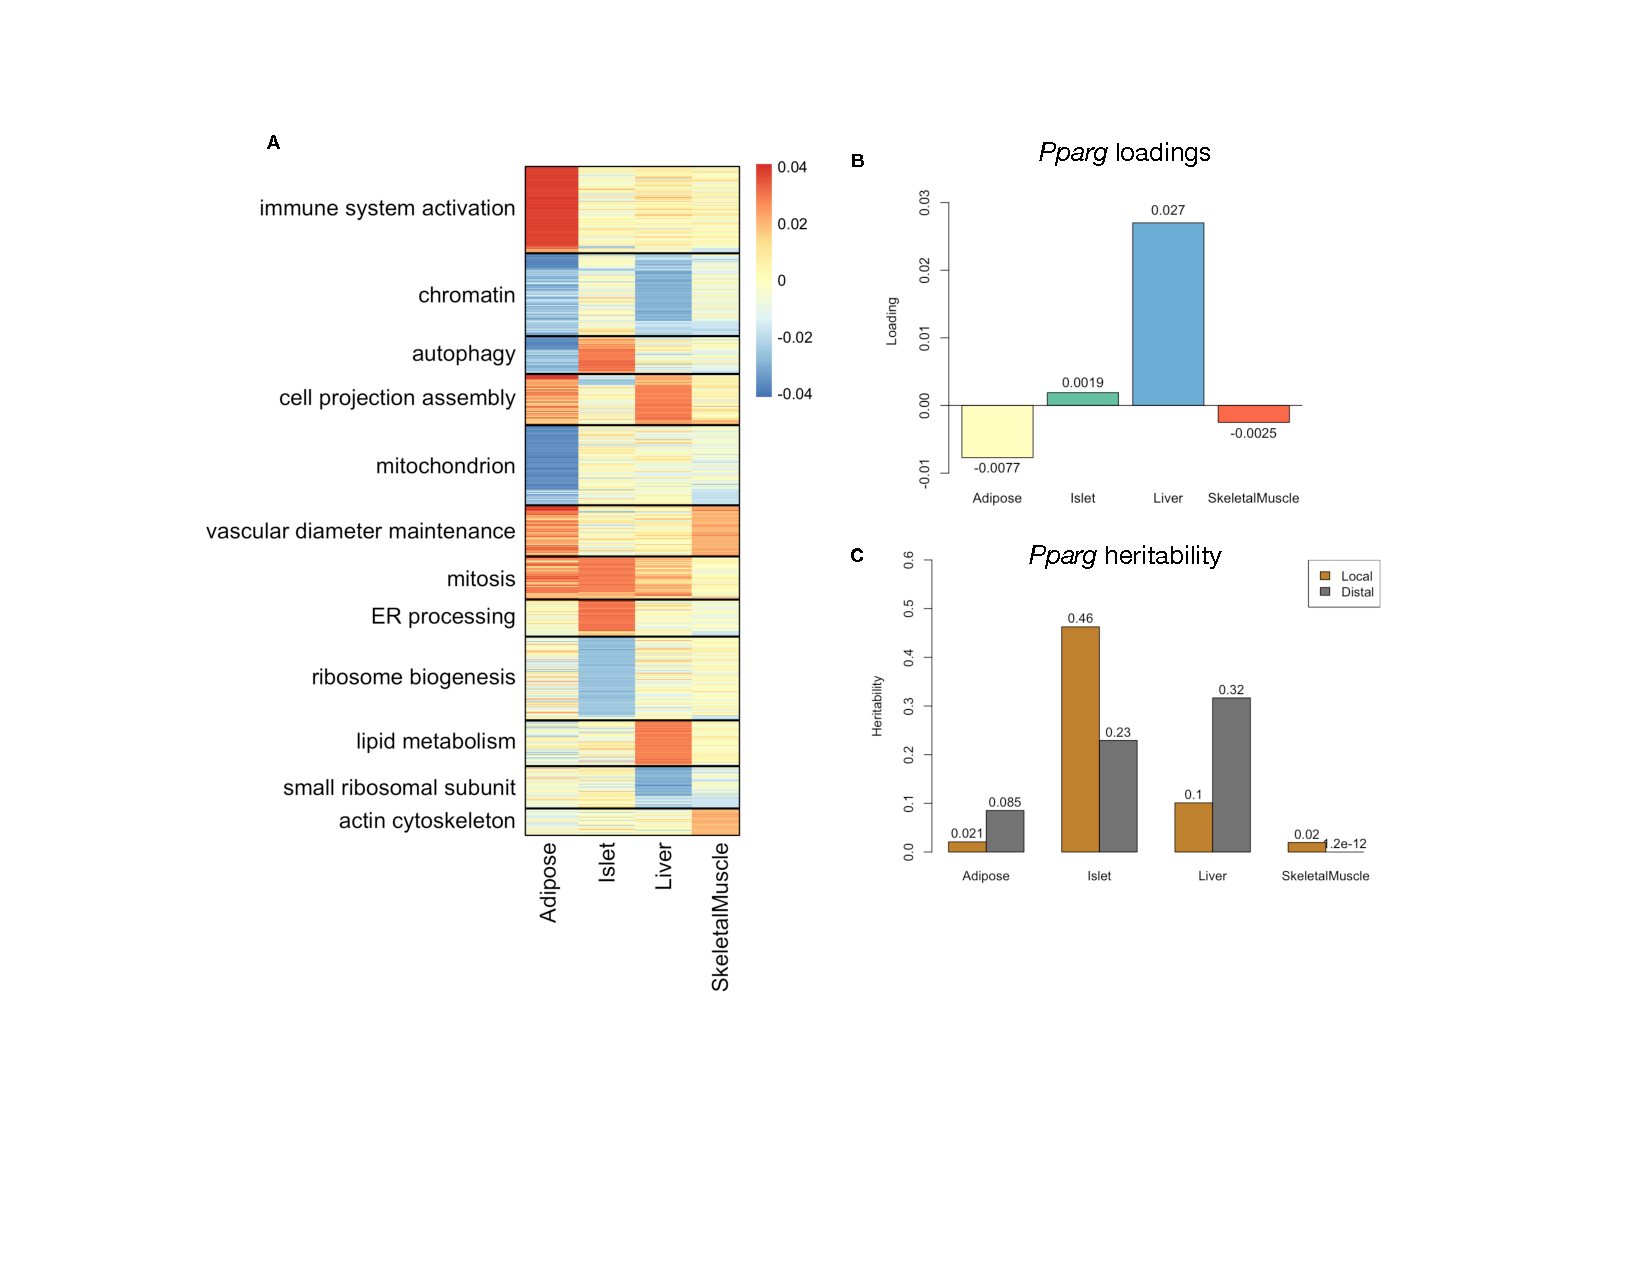
\includegraphics[width=\textwidth]{Figures/Fig6_TOA.pdf} 
\caption{Tissue-specific transcriptional programs were associated 
with obesity and insulin resistance. \textbf{A} Heat map showing 
the loadings of all transcripts with loadings greater than 2.5 
standard deviations from the mean in any tissue. The heat map was 
clustered using k medoid clustering. Functional enrichments of each 
cluster are indicated along the left margin. \textbf{B} Loadings for 
\textit{Pparg} in different tissues. \textbf{C} Local and distal of 
\textit{Pparg} expression in different tissues.
}
\label{fig:toa}
\end{figure}

\begin{figure}[ht!]
\includegraphics[width=\textwidth]{Figures/Fig7_CC_Prediction.pdf} 
\caption{Transcription, but not local genotype, predicts 
phenotype in the CC-RIX. \textbf{A.} Workflow showing procedure 
for translating HDMA results to an independent population of mice. 
\textbf{B.} Relationships between the predicted metabolic disease
index (MDI) and measured body weight in the CC-RIX. The left column 
shows the predictions using measured transcripts. The right column 
shows the prediction using transcript levels imputed from local 
genotype. Gray boxes indicate measured quantities, and blue boxes 
indicate calculated quantities. The dots in each panel represent 
individual CC-RIX strains. The gray lines show the standard deviation 
on body weight for the strain.
}
\label{fig:cc_prediction}
\end{figure}

\begin{figure}[ht!]
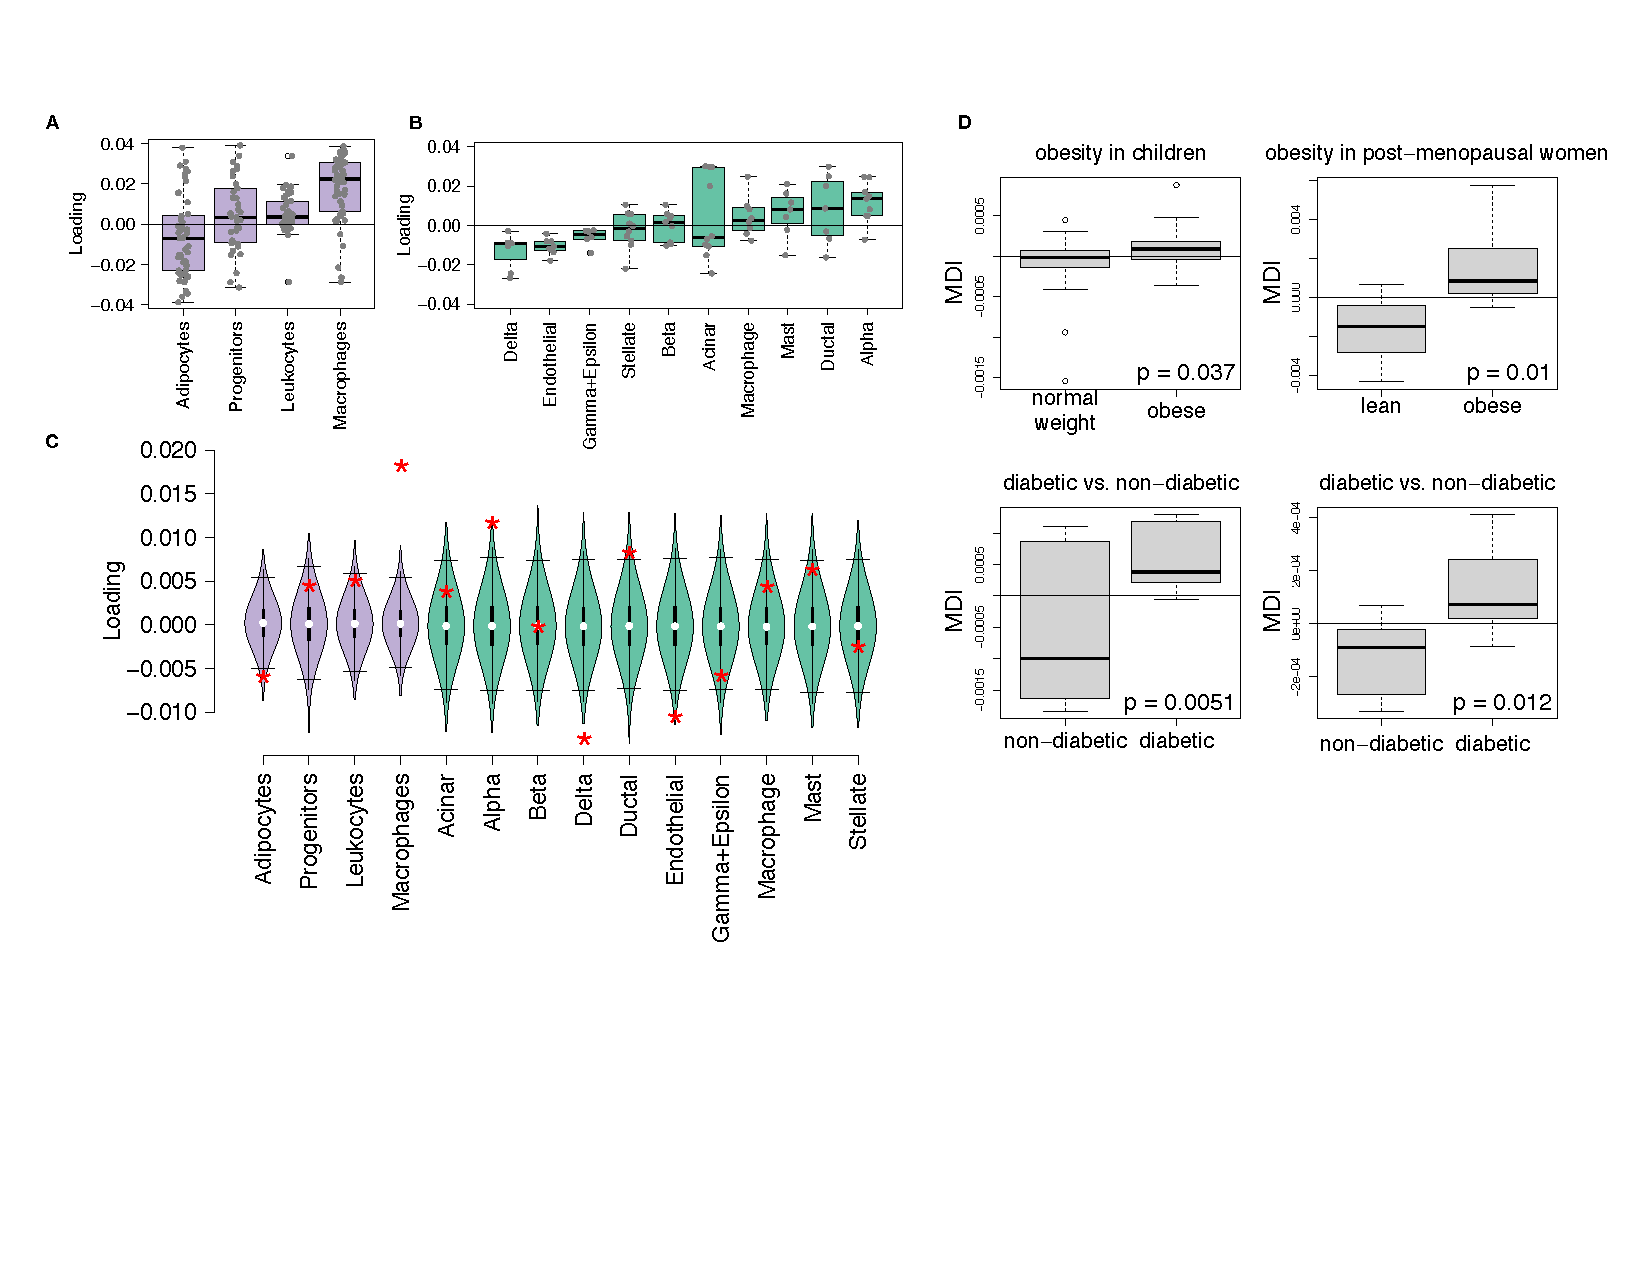
\includegraphics[width=\textwidth]{Figures/Fig8_Human_Translation.pdf} 
\caption{HDMA results translate to humans. \textbf{A.} Distribution of 
loadings for cell-type-specific transcripts in adipose tissue. \textbf{B.} 
Distribution of loadings for cell-type-specific transcripts in pancreatic 
islets. \textbf{C.} Null distributions for the mean loading of 
randomly selected transcripts in each cell type compared with the observed 
mean loading of each group of transcripts (red asterisk). \textbf{D.} 
Predictions of metabolic phenotypes in four adipose transcription data 
sets downloaded from GEO. In each study the obese/diabetic patients were 
predicted to have greater MDI than the lean/non-diabetic 
patients based on the HDMA results from DO mice.
}
\label{fig:human_translation}
\end{figure}

\end{document}
